In this section I explore four methods of dimensionality reduction on both of my datasets.

\subsection{Principal Components Analysis}\label{subsec:principal-components-analysis}
For principal component analysis I chose to vary the number of components to explain variance, and collected their resulting eigenvalues to better understand this DR technique.
Below is a table of results for both data sets.
\begin{center}
    \begin{tabular}{|c| c |c|}
        \hline
        & Minimum Components to Explain 99.9\% Variance & Eigenvalues                               \\
        \hline
        \hline
        Dataset 1 & 2                                             & [11320901200.524, 54484006.504]           \\
        \hline
        Dataset 2 & 4                                             & [65088.565, 37527.175, 4525.986, 106.278] \\
        \hline
    \end{tabular}
\end{center}
Two features explain 100\% of the variance in the data in the case of PCA for dimensionality reduction, and four features explain
99.9\% of the variance in the case of the second dataset.
In the case of dataset one the eigenvalues are very large which would seem to imply that the data are close together and
the are being multiplied by a large number to separate.
By contrast, data set two seems to have more components needed to explain the variance and each of those as a slightly smaller eigenvalue.
Figures~\ref{Fig:PCA DS1} and~\ref{Fig:PCA DS2} show the projection of the transformed data according to their principal
components for the first two features (to allow for plotting).
\begin{figure}
    \begin{minipage}{0.5\textwidth}
        \centering
        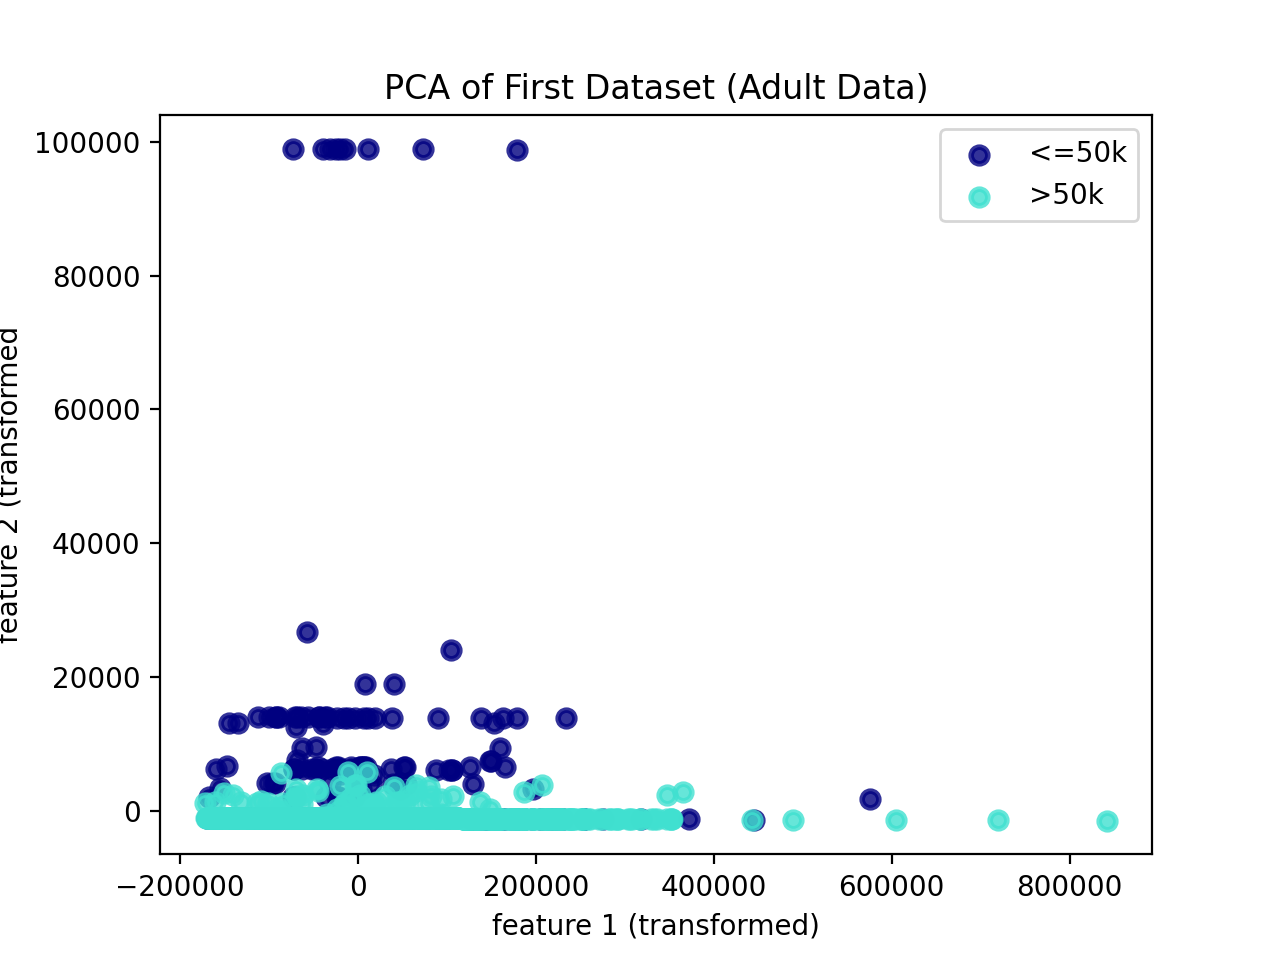
\includegraphics[width=.9\linewidth]{pcads1.png}
        \caption{DS1 Projection via PCA}\label{Fig:PCA DS1}
    \end{minipage}\hfill
    \begin{minipage}{0.5\textwidth}
        \centering
        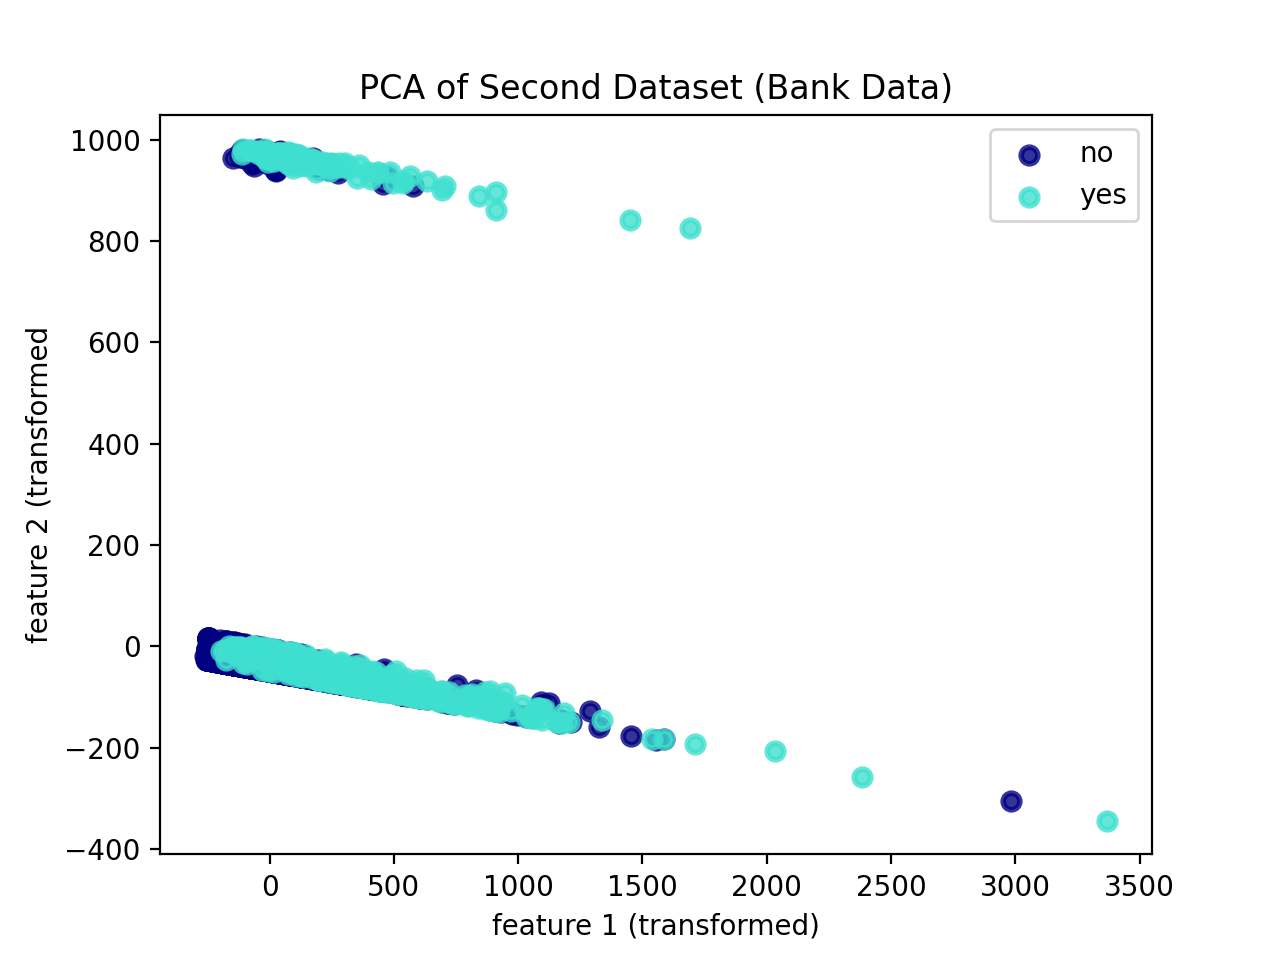
\includegraphics[width=.9\linewidth]{pcads2.png}
        \caption{DS1 Projection via PCA}\label{Fig:PCA DS2}
    \end{minipage}
\end{figure}

\subsection{Independent Components Analysis}\label{subsec:independent-components-analysis}
Similar to the previous I also attempted to search for the best number of independent "source components" for each dataset.
According to Carsten Klein\cite{klein_2019}
"An interesting thing about two independent, non-Gaussian signals is that their sum is more Gaussian than any of the source signals.
Therefore we need to optimize W in a way that the resulting signals of Wx are as non-Gaussian as possible."
In other words, using a measurement like Kurtosis we can compare the "Gaussianity" of different ICA runs.
Since the normal distribution (Gaussian) has a kurtosis of 3, we are searching for ICA components with kurtosis of $<$ 3.
In order to reduce the covariance of the feature vectors as much as possible (to in effect ensure they were independent
components, I elected to whiten the feature space before processing.)
Below is a table depicting the n-components selected for each dataset and the resulting Kurtosis.
\begin{figure}
    \begin{minipage}{0.5\textwidth}
        \centering
        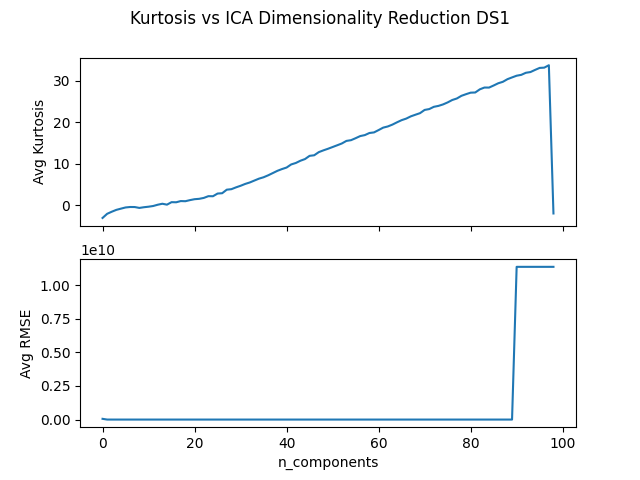
\includegraphics[width=.9\linewidth]{icads1.png}
        \caption{ICA Kurtosis vs RCError DS1}\label{Fig:ICA DS1}
    \end{minipage}\hfill
    \begin{minipage}{0.5\textwidth}
        \centering
        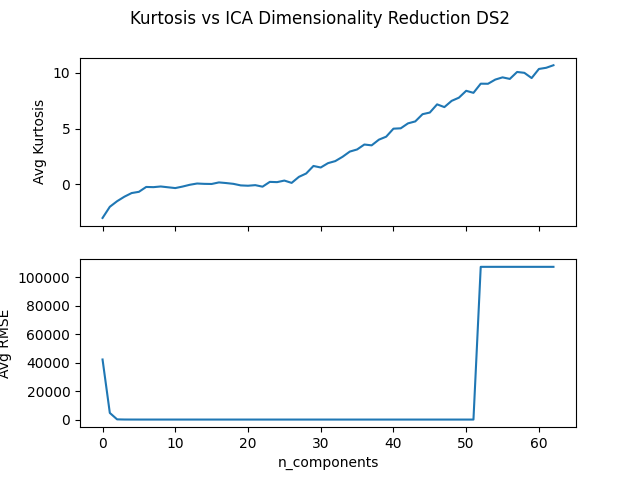
\includegraphics[width=.9\linewidth]{icads2.png}
        \caption{ICA Kurtosis vs RCError DS2}\label{Fig:ICA DS2}
    \end{minipage}
\end{figure}
Looking at figures~\ref{Fig:ICA DS1} and~\ref{Fig:ICA DS2} we can see the relationship between the number of components (the dimensions reduced to)
and both Kurtosis and Reconstruction Error (as measured by mean squared error).
Similar to PCA, for small values of n\_components reconstruction error quickly approaches zero where the kurtosis gradually
rises for each additional component.
This would seem to suggest that for $n=2$ (Dataset 1) and $n=4$ (Dataset 2) we reach the optimal tradeoff between treating
each source attribute "as a seperate mixed signal" and reducing RC error (the obvious bias in DR being that we want n to be as
small as possible.)
With respect to each dataset the meaningfulness of this result is that it is possible to reconstruct the distribution with
significantly less data than the many more attributes which generated the original.


\subsection{Randomized Projection}\label{subsec:randomized-projection}
Randomized projections allowed me to generate random dimensionality reduction transformations from the data.
I chose to repeat this process 10 times for each dataset and to utilize a Gaussian Randomized projection such that each
feature was itself equally likely to be a part of the final dimensionally reduced output.
Along with repeating each experiment I chose to vary the number of components as I did in other experiments to search
for an optimal reconstruction error.
Perhaps unsurprisingly looking at figures~\ref{Fig:RP DS1} and~\ref{Fig:RP DS2} we can see that for larger values of
\texttt{n\_components} the reconstruction error was lower.
The oscillations in the graph can be explained by the fact that the random projections can increase or decrease the RCError
by small amounts.
There was a significant amount of variance between runs as shown in the table~\ref{RP Var}.
Dataset 1 had much more variance than dataset 2 during randomized projection runs.
This is most likely due to the 30+ additional features in the space for which a random selection/transformation needed
to be made.
\begin{center}\label{RP Var}
    \begin{tabular}{|c| c |c|}
        \hline
        & Variance               & Standard Deviation \\
        \hline
        \hline
        Dataset 1 & 5.4456097845336664e+16 & 233358303.57057506 \\
        \hline
        Dataset 2 & 34540925361.18495      & 185851.89092711688 \\
        \hline
    \end{tabular}
\end{center}
\begin{figure}
    \begin{minipage}{0.5\textwidth}
        \centering
        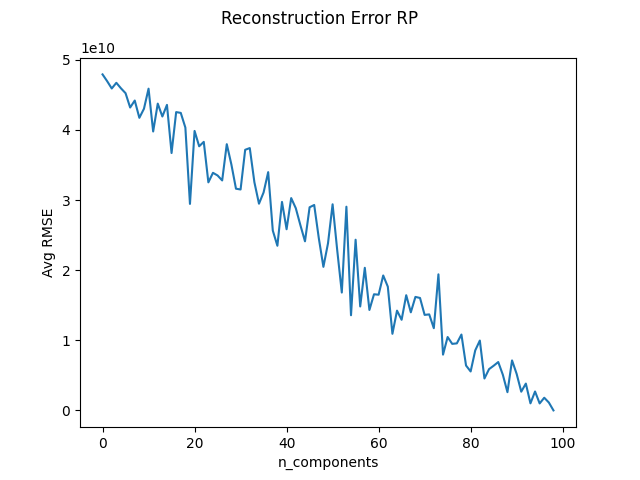
\includegraphics[width=.9\linewidth]{rpds1.png}
        \caption{RCError RP DS1}\label{Fig:RP DS1}
    \end{minipage}\hfill
    \begin{minipage}{0.5\textwidth}
        \centering
        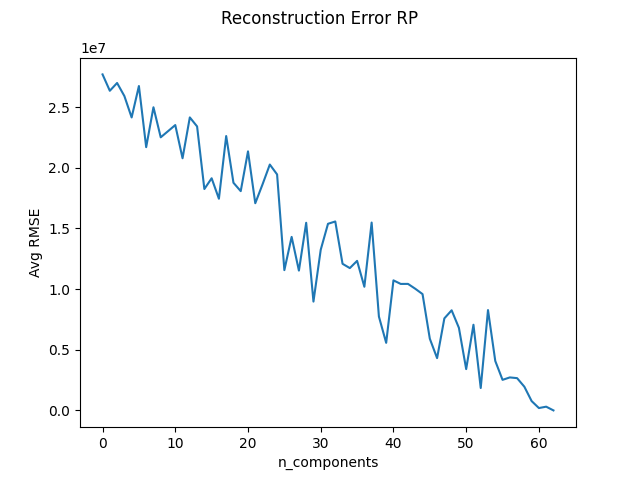
\includegraphics[width=.9\linewidth]{rpds2.png}
        \caption{RCError RP DS1}\label{Fig:RP DS2}
    \end{minipage}
\end{figure}

\subsection{Linear Discriminant Analysis}\label{subsec:linear-discriminant-analysis}
For my final dimensionality reduction technique, I chose to use linear discriminant analysis.
Due to the fact that each of my problems are binary classification, and while not linearly seperable (otherwise accuracy would be better,)
a linear decision boundary with Bayesian conditional density would allow me to reduce the dimensionality of the dataset similar
to PCA in the direction of the largest discriminant.
However the difference here is the introduction of a priori information in the form of class labels.
The number of components had to be $min(num\_features, unique\_labels - 1)$ which in my case was $1$ for both datasets given
that they were both binary classification problems.
Since LDA takes into account class labels I chose (similar to classifiers) to split the data between a test/training set (25/75\% respectively.)
After the transformation I opted to classify the remainder of instances, below is the result on test data.
\begin{center}
    \begin{tabular}{|c| c |}
        \hline
        & Accuracy \\
        \hline
        \hline
        Dataset 1 & 82.86\%  \\
        \hline
        Dataset 2 & 91.17\%  \\
        \hline
    \end{tabular}
\end{center}
As you can see these results are comparable to the accuracy scores of some of the better trained classifiers from assignment 1.
This I believe speaks to the power of LDA being able to consider apriori information in constructing the DR projection.
Unfortunately given that there was only one value for \texttt{n\_components} I cannot compare reconstruction error over time,
but given the positive results, I don't think that the reconstruction error would be very high.